\chapter{Directed graphs}\label{digraphs_chap}
%\section{Digraphs}\label{digraphs_sec}

%\hyperdef{directed}{graph}

\term{Directed graphs}, \term{digraphs} for short, provide a handy way
to represent how things are connected together and how to get from one
thing to another by following the connections.  They are usually
pictured as a bunch of dots or circles with arrows between some of the
dots as in Figure~\ref{fig:6EB}.  The dots are called \emph{nodes} (or
\emph{vertices}) and the lines are called \emph{directed edges} or
\term{arrows}, so the digraph in Figure~\ref{fig:4N6E} has 4 nodes and
6 directed edges.

\begin{figure}

\graphic{Fig_EB}

\caption{A 4-node directed graph with 6 edges.}

\label{fig:4N6E}

\end{figure}

\iffalse

One common situation where they naturally come up is in task
scheduling, where nodes represent tasks to be completed and arrows
indicate which tasks must be completed before others can begin.  For
example, Figure~\ref{6-3_subjects} shows the prerequisite structure
among MIT computer science subjects.

\begin{figure}

\includegraphic[5in]{6-3_dag}

\caption{Subject prerequisites for MIT Computer Science (6-3) Majors}

\label{6-3_subjects}

\end{figure}
\fi

Digraphs appear everywhere in computer science.  In
section~\ref{comm_net_sec}, we'll use digraphs are used to describe
\idx{communication nets} for routing data packets.  The digraph in
Figure~\ref{fig:6switchnet} has three ``in'' nodes (pictured as little
squares) representing locations where packets may arrive at the net,
the three ``out'' nodes representing destination locations for
packets, and the remaining six nodes (pictured with little circles)
represent switches.  The 16 edges indicate paths that packets can take
through the router.

\begin{figure}

\graphic{MQ_oct31_network}

\caption{A 6-switch packet routing digraph.}

\label{fig:6switchnet}

Another digraph example, is the hyperlink structure of the World Wide
Web.  Letting the vertices $x_1, \ldots, x_n$ correspond to web pages
and using arrows to indicate when one page has a hyperlink to another,
yields a digraph like the one Figure~\ref{webpage-links}.  In the
graph of the real World Wide Web, $n$ would be a number in the
billions and probably even the trillions.  At first glance, this graph
wouldn't seem to be very interesting.  But in 1995, two students at
Stanford, \index{Page, Larry} Larry Page and index{Brin, Sergey}
Sergey Brin ultimately became multibillionaires from the realization
of how useful the structure of this graph could be in building a
search engine.  So pay attention to graph theory, and who knows what
might happen!

\iffalse

and in the following graph the vertices $x_1, \ldots, x_n$ correspond
to web pages and $\diredge{x_i}{x_j}$ is a directed edge when page
$x_i$ contains a hyperlink to page $x_j$.
\fi


\begin{figure}

\graphic{randomWalkFigs/webGraph}

\caption{Links among Web Pages}

\label{webpage-links}

\end{figure}


\subsection{Digraph Walks and Paths}

\begin{definition}\label{graphdef}
  A \term{directed graph} $G$ consists of a nonempty
  set,~$\vertices{G}$, called the \term{vertices} of~$G$, and a set
  $\edges{G}$ called the \term{edges} of $G$.  An element of
  $\vertices{G}$ is called a \term{vertex}.  A vertex is also called a
  \term{node}; the words ``vertex'' and ``node'' are used
  interchangeably.  An element of $\edges{G}$ is called a
  \term{directed edge}.  A directed edge is also called an ``arrow''
  or simple an ``edge.''  A directed edge \index{start
    vertex}{\emph{starts}} at some vertex $u$ and \index{end
    vertex}{\emph{ends}} at some vertex, $v$.  Such an edge can be
  represented by the ordered pair $(u,v)$.  The notation
  $\diredge{u}{v}}$ denotes this edge.
\end{definition}

There is nothing new in Definition~\ref{graphdef} except for a lot of
vocabulary.  Formally, a digraph $G$ is the same as a binary relation
the set, $V = \vertices{G}$ ---that is, a relation whose domain and
codomain are the same set, $V$.  In fact we've already referred to the
arrows in a relation $G$ as the ``graph'' of $G$.
For example, the \idx{divisibility
  relation} on the integers in the interval $[1,12]$ could be pictured
by the digraph in Figure~\ref{fig:divisibility-digraph}.

\begin{figure}
\graphic{divisibility}
\caption{The Digraph for Divisibility on $\set{1,2,\dots,12}$.}
\label{fig:divisibility-digraph}
\end{figure}

Picturing digraphs with points and arrows makes it natural to talk
about following taking a walk along successive edges through the
graph.  For example, in the digraph of
Figure~\ref{fig:divisibility-digraph}, a walk might start at vertex 1,
successively follow the edges from vertex 1 to vertex 2, from 2 to 4,
from 4 to 12, and then from 12 to 12 twice (or as many times as you
like).  The obvious way to represent a walk is with the sequence of
sucessive vertices it went through, in this case:
\[
1,2,4,12,12,12.
\]
However, a walk is represented by an alternating sequence of
successive vertices and edges, so this walk would formally be
\begin{equation}\label{walk12412}
1,\diredge{1}{2}, 2, \diredge{2}{4}, 4,\diredge{4}{12}, 12,
\diredge{12}{12}, 12,\diredge{12}{12}, 12.
\end{equation}\
The redundancy of this definition is enough to make any computer
scientist cringe, but it does make it easy to talk about how many
times vertices and edges occur on the walk.  Here is a formal
definition:

\begin{definition}\label{def:digraph-walks}
A \term{walk in a digraph}, $G$, is an alternating sequence of
vertices and edges that begins with a vertex, ends with a vertex, and
such that for every edge $\digraph{u}{v}$ in the walk, vertex $u$ is
the element just before the edge, and vertex $v$ is the next element
after the edge.

So a walk, \walk{v}, is a sequence of the form
\[
\walk{v} \eqdef v_0, \diredge{v_0}{v_1}, v_1, \diredge{v_1}{v_2}, v_2, \dots, \diredge{v_{k-1}}{v_k}, v_k
\]
where $\diredge{v_i}{v_{i+1}} \in \vertices{G}$ for $i \in [0,k)$.
  The walk is said to \emph{start} at $v_0$, to \emph{end} at $v_k$,
  and the \emph{length}, $lnth{\walk{v}}$ of the walk is defined to be
  $k$.  The walk is a \emph{path} iff all the $v_i$'s are different,
  that is, if $i \neq j$, then $v_i \neq v_j$.
\end{definition}
Note that a single vertex counts as length zero walk that begins and
ends at itself.

If you walk for a while, stop for a rest at some vertex, and then
continue walking, you have broken a walk into two parts.  For example,
stopping to rest after following two edges in the walk~\ref{walk12412}
through the divisibility graph breaks the walk into the walk
\begin{equation}\label{startwalk124}
1,\diredge{1}{2}, 2, \diredge{2}{4}, 4
\end{equation}
from 1 to 4, and the walk
\begin{equation}\label{endwalk412}}
4,\diredge{4}{12}, 12, \diredge{12}{12}, 12,\diredge{12}{12}, 12.
\end{equation}
from 4 to 12, and we'll say the whole walk~\ref{walk12412} is the
\term{merge} of the walks~\ref{startwalk124} and~\ref{endwalk412}.  In
general, if a walk $\walkv{f}$ ends with a vertex, $v$, and a walk
$\walkv{r}$ starts with the same vertex, $v$, we'll say that the
\term{merge} of $\merge{\walkv{f}}{\walkv{r}}$ is the walk that starts
with $\walkv{f}$ and continues with $\walkv{r}$.\footnote{It's
  tempting say the \emph{merge} is the \idx{concatentation} of the two
  walks, but that wouldn't quite be right because the vertex $v$ would
  appear twice in a row where the walks meet.}  Two walks can only be
merged if the first end with the same vertex, $v$, that the second one
starts with.  Sometimes its useful to name the node $v$ where the
walks merge; we'll use the notation $\catv{\walkv{f}}{v}{\walkv{r}}$
to describe the merge of a walk $\walkv{f}$ that ends at $v$ with a
walk $\walkv{r}$ that begins at $v$.

\iffalse
 Here's a precise definition:
\begin{definition}
If a walk $\walkv{f}$ ends at a vertex $v$ and a walk $\walkv{r}$
begins at the same vertex $v$, then the \term{$v$-merge} of
$\walkv{f}$ with $\walkv{r}$, written,
\[
\catv{\walkv{f}}{v}{\walkv{r}},
\]
is the walk whose vertex sequence is the vertex sequence of
$\walkv{f}$ concatenated with the vertex sequence of $\walkv{r}$
without its initial $v$.  That is, if
\begin{align*}
\walkv{r} & = v\,\vec{\alpha},
\end{align*}
for some finite sequence $\vec{\alpha}$ of vertices,
then
\[
\catv{\walkv{f}}{v}{\walkv{r}} \eqdef  \walkv{f}\alpha.
\]
\end{definition}
\fi

A useful consequence of this definition is that
\begin{lemma}\label{sumoflengths}
\lnth{\merge{\walkv{f}}{\walkv{r}} = \lnth{\walkv{f}} + \lnth{\walkv{r}}.
\end{lemma}
We'll shortly get further useful mileage out of walking this
way.

\subsection{Finding a Path}
If you were trying to walk somewhere quickly, you'd know you were in
trouble if you came to the same place twice.  This is actually a basic
theorem of graph theory.

\begin{theorem}\label{simplepath}
The shortest walk between a pair of vertices is a path.
\end{theorem}

\begin{proof}
  If there is a walk from vertex $u$ to $v$, there must, by the
  Well Ordering Principle, be a minimum length walk $\walkv{w}$ from $u$
  to~$v$.  We claim $\walkv{w}$ is a path.

  To prove the claim, suppose to the contrary that $\walkv{w}$ is not a
  path, namely, some vertex $x$ occurs twice on this walk.  That is,
\[
\walkv{w} = \catv{\catv{\walkv{e}}{x}{\walkv{f}}}{x}{\walkv{g}}
\]
for some walks $\walkv{e}, \walkv{f}, \walkv{g}$ where the length of
$\walkv{f}$ is positive.  But then deleting $\walkv{f}$ yields is a
strictly shorter walk
\[
\catv{\walkv{e}}{x}{\walkv{g}}
\]
from $u$ to $v$, contradicting the minimality of $\walkv{w}$.
\end{proof}

Actually, we proved something stronger:
\begin{corollary}\label{pathlewalk}
For any walk of length $k$ in a graph, there is a path of length
\emph{at most} $k$ with the same endpoints.  Moreover, the shortest
walk between a pair of vertices is, in fact, a path.
\end{corollary}

\begin{editingnotes}
Distance properties below \arm{inserted by arm}
\end{editingnotes}

\begin{definition}
  The \index{distance!between vertices} \emph{distance} $\dstuv{u}{v}$
  between vertices $u,v$ in a graph is the length of a shortest walk
  from $u$ to $v$.
\end{definition}

As would be expected, this definition of distance satisfies:
\begin{lemma}\label{lem:tri-ineq} [The Triangle Inequality]
\[
\dstuv{u}{v} \leq \dstuv{u}{x} + \dstuv{x}{v}
\]
for all vertices $u,v,x$ with equality holding iff $x$ is on a shortest
path from $u$ to $v$.
\end{lemma}
Of course you may expect this property to be true, but it really
should be proved, since distance has a technical definition and its
properties can't be taken for granted.

\begin{editingnotes}
  Maybe leave all or part the following proof to a problem?
\end{editingnotes}

\begin{proof}
  To prove the inequality, suppose $\walkv{f}$ is a shortest path from
  $u$ to $x$ and $\walkv{r}$ is a shortest path from $x$ to $v$.  Then
  by Lemma~\ref{sumoflengths} $\catv{\walkv{f}}{x}{\walkv{r}}$ is a
  path of length $\dstuv{u}{x} + \dstuv{x}{v}$ from $u$ to $v$, so
  this sum is an upper bound on the length of the shortest path from
  $u$ to $v$.

  To prove the ``iff'' from left to right, suppose $\dstuv{u}{v} =
  \dstuv{u}{x} + \dstuv{x}{v}$.  Then taking a shortest path from $u$ to
  $x$ followed by a shortest path from $x$ to $w$ yields a path of whose
  length is $\dstuv{u}{x} + \dstuv{x}{v}$ which by assumption equals
  $\dstuv{u}{v}$. So this is a shortest path containing $x$.

  To prove the ``iff'' from right to left, suppose vertex $x$ is on a
  shortest path $\walkv{w}$ from $u$ to $v$, namely, $\walkv{w}$ is a
  shortest path of the form $\catv{\walkv{f}}{x}{\walkv{r}}$.  The
  path $\walkv{f}$ must be a shortest path from $u$ to $x$; otherwise
  replacing $\walkv{f}$ by a shorter path from $u$ to $x$ would yield
  a shorter path from $u$ to $v$ than $\walkv{w}$.  Likewise from
  $\walkv{r}$ must be a shortest path from $x$ to $v$.  So
  $\dstuv{u}{v} = \abs{\walkv{w}} = \abs{\walkv{f}} + \abs{\walkv{r}}
  = \dstuv{u}{x} + \dstuv{x}{v}$.
  
\end{proof}

\subsection{Adjacency Matrices}
If a graph, $G$, has $n$ vertices, $v_0,v_1,\dots, v_{n-1}$, a useful
way to represent it is with a $n \times n$ matrix of zeroes and ones
called its \term{adjacency matrix}, $A_G$ of the graph.  The $ij$th
entry, $(A_G)_{ij}$, of the adjacency matrix is 1 if there is an edge
from vertex $v_i$ to vertex $v_j$, and 0 otherwise.  That is
\[
(A_G)_{ij} \eqdef \begin{cases} 1 & \text{if } \diredge{v_i}{v_j} \in
  \vertices{G},\\
0 & \text{otherwise}.
\end{cases}

For example, let $H$ be the 4-node the graph shown in
Figure~\ref{Fig_EB}.  Then its adjacency matrix $A_H$ is the $4 \times
4$ matrix:
\[
A_H =\begin{array}{c|cccc|}
  &  a & b & c & d \\ \hline
a &  0 & 1 & 0 & 1 \\
b &  0 & 0 & 1 & 1 \\
c &  0 & 1 & 0 & 0 \\
d &  0 & 0 & 1 & 0
\end{array}
\]

A payoff of this representation is that we can use matrix powers to
count numbers of walks between vertices.  For example, there are two
length two walks between verices $a$ and $c$ in the graph $H$, namely
\begin{align*}
a\, \diredge{a}{b}\, b \diredge{b}{c}\,  c\\
a\, \diredge{a}{db}\, d \diredge{d}{c}\,  c
\end{align*}
and these are the only length two walks from $a$ to $c$.  Also, there
is exactly one length 2 walk from $b$ to $c$ and exactly one length 2
walk from $c$ to $c$ and from $d$ to $b$, and these are the only
length 2 walks in $H$.  It turns out we could have read these counts
from the entries in the matrix $(A_H)^2$:
\[
(A_H)^2 = \begin{array}{c|cccc|}
  &  a & b & c & d \\ \hline
a &  0 & 0 & 2 & 0 \\
b &  0 & 0 & 1 & 0 \\
c &  0 & 0 & 1 & 0 \\
d &  0 & 1 & 0 & 0
\end{array}
\]

\iffalse
If $G$ is a weighted graph with edge weights given by $w: E \to
\reals$, then the adjacency matrix for~$G$ is $A_G = \{ a_{ij} \}$
where
\begin{equation*}
    a_{ij} = \begin{cases}
                w(\edge{v_i}{v_j}) & \text{if $\edge{v_i}{v_j} \in E$} \\
                0                 & \text{otherwise.}
              \end{cases}
\end{equation*}
\end{definition}

For example, Figure~\ref{fig:adjacency_matrix} displays the adjacency
matrices for the graphs shown in Figures~\ref{fig:isomorphism}(a)
and~\ref{fig:weighted_graph} where $v_1 = a$, $v_2 = b$, $v_3 = c$,
and $v_4 = d$.
\fi

More generally, the matrix $(A_G)^k$ provides a count of the number of
length $k$ walks between vertices in any digraph, $G$, as we'll now
explain.

\begin{definition}
  The length $k$ \term{walk counting matrix} for an $n$-vertex graph $G$
  is the $n \times n$ matrix $C$ such that
\begin{equation}\label{def:walk_matrix}
C_{uv} \eqdef
\begin{cases}  & \text{if there is a length $k$ walk from vertex
                     $u$ to vertex $v$},\\
              0 & \text{otherwise}.
\end{cases}
\end{equation}
\end{definition}

So the length $1$ walk counting matrix for $G$ is precisely its
adjacency matrix $A_G$.

\begin{theorem}\label{thm:CkDm}
 If $C$ is length $k$ walk counting matrix for a graph $G$, and $D$ is
 the length $m$walk counting matrix, then $CD$ is the length $k+m$
 walk counting matrix for $G$.
\end{theorem}

According to this theorem, the square $(A_G)^2$ of the adjacency
matrix is the length 2 walk counting matrix for $G$.  Applying the
theorem again to $(A_G)^2A_G$, shows that the length 3 walk counting
matrix is $(A_G)^3$.  More generally, it follows by induction that
\begin{corollary}\label{AGklenk}
The length $k$ counting matrix

\end{corollary}
 $(A_G)^k$ is the length $k$ walk
counting matrix.  In other words, you can determine the number of
length~$k$ walks between any pair of vertices simply by computing the
$k$th power of the adjacency matrix!  That's pretty amazing.  \iffalse

For example, the first three powers of the adjacency matrix for the
graph in Figure~\ref{fig:5AD} are:
\begin{align*}
    A &= \begin{pmatrix}
            0 & 1 & 1 & 1 \\
            1 & 0 & 1 & 0 \\
            1 & 1 & 0 & 1 \\
            1 & 0 & 1 & 0
         \end{pmatrix} & % \\[\medskipamount]
  A^2 &= \begin{pmatrix}
            3 & 1 & 2 & 1 \\
            1 & 2 & 1 & 2 \\
            2 & 1 & 3 & 1 \\
            1 & 2 & 1 & 2
         \end{pmatrix} & % \\[\medskipamount]
  A^3 &= \begin{pmatrix}
            4 & 5 & 5 & 5 \\
            5 & 2 & 5 & 2 \\
            5 & 5 & 4 & 5 \\
            5 & 2 & 5 & 2
         \end{pmatrix}
\end{align*}

Sure enough, $(A^3)_{14}$ is $5$, which is the number of length~3 walks
from~$v_1$ to~$v_4$.  And $(A^3)_{24} = 2$, which is the number of
length~3 walks from $v_2$ to~$v_4$.  
\fi

By proving the theorem, we'll discover why it is true and thereby
uncover the relationship between matrix multiplication and numbers of
walks.

\begin{editingnotes}
\arm{new proof replacing induction proof by ftl}
\end{editingnotes}

\begin{proof}[Proof of Theorem~\ref{thm:CkDm}]
  Any length $k+m$ walk between vertices $u$ and $v$ begins with a
  length $k$ walk starting at $u$ and ending at some vertex,
  $w$, followed by a length $m$ walk starting at $w$ and ending at $v$.  So
  the number of length $k+m$ walks from $u$ to $v$ that go through
  $w$ at the $k$th step equals the number $P_{uw}$ of length $k$ walks
  from $u$ to $w$, times the number $Q_{wv}$ of length $m$ walks from $w$
  to $v$.  We can get the total number of length $k+m$ walks from $u$
  to $v$ by summing, over all possible vertices $w$, the number of such
  walks that go through $w$ at the $n$th step.  In other words,
\begin{equation}\label{ln+nuv}
\text{\# length $k+m$ walks between $u$ and $v$} =
              \sum_{w \in \vertices{G}} C_{uw}\cdot D_{wv}
\end{equation}
But the right hand side of~\eqref{ln+nuv} is precisely the definition of
$(CD)_{uv}$.  Thus, $CD$ is indeed the length $k+m$ walk counting matrix.
\end{proof}



\subsubsection{Minimum Weight Path  Matrices}
The relation between powers of the adjacency matrix and numbers of
walks is cool (to us math nerds at least),
\begin{editingnotes}
\arm{math nerds? \smiley}
\end{editingnotes}
but a much more important
problem is finding \index{graph!shortest path} shortest paths between
pairs of nodes in a graph.  For example, when you drive home for vacation,
you generally want to take the shortest-time route.  It turns out that
shortest paths---even in weighted graphs---can be determined in pretty
much the same way that numbers of paths were counted using powers of the
connection matrix.

\begin{definition}\label{def:5H}
  The \index{path!weight of}\term{weight of a walk} \index{weighted graph,
    path weight} in a \idx{weighted graph} is the sum of the weights of
  the successive edges in the walk.
\end{definition}

\begin{editingnotes}
\arm{cut}
There is good news and bad news to report on this front.  The good
news is that it is not very hard to find a shortest path.  The bad
news is that you can't win one of those million dollar prizes for
doing it.

In fact, there are several good algorithms known for finding a shortest
path between nodes $u$ and $v$ in an $n$-node graph $G$.  The simplest to
explain (but not quite the fastest) is to compute \arm{revised to include
  stopping condition at $n$} the successive powers of $A_G$ one by one up
to the $n$th, watching for the first power at which the $uv$th entry is
nonzero.  That's because Theorem~\ref{thm:CkDm} implies that the length of
the shortest path, if any, between $u$ and~$v$ will be the smallest
value~$k$ for which $(A_G)_{uv}^k$ is nonzero, and if there is a shortest
path, its length will be $\leq n$.
\end{editingnotes}

\begin{definition}
  The \term{minimum weight matrix} for length $k$ walks in an $n$-vertex
  graph $G$ is the $n \times n$ matrix $W$ such that for $u,v \in \vertices{G}$,
\begin{equation}\label{def:weight_matrix}
W_{uv} \eqdef
\begin{cases} w & \text{if $w$ is the minimum weight among length $k$
                            walks from $u$ to $v$},\\
              \infty & \text{if there is no length $k$ walk from $u$ to $v$}.
\end{cases}
\end{equation}
\end{definition}

So the minimum weight matrix for length $1$ walks in a weighted graph $G$
is precisely its adjacency matrix $A_G$.  Now for the purpose of finding
minimum weight walks, we'll modify the definition of matrix
multiplication, replacing multiplication of elements by addition, and the
sum of the products by the minimum.

\begin{definition}\label{def:minplus}
  The $\minplus$ product of two $n\times n$ matrices $W$ and $M$ with
  entries in $\reals\union \set{\infty}$ is the $n \times n$ matrix
  $W\minplusop M$ whose $ij$ entry is
\[
(W\minplusop M )_{ij} \eqdef \min \set{W_{ik} + M_{kj} \suchthat 1 \leq k \leq n}\, .
\]
\end{definition}

\begin{theorem}\label{thm:weightmatrix-min+}
  If $W$ is the minimum weight matrix for length $k$ walks in a weighted
  graph $G$, and $M$ is the minimum weight matrix for length $m$ walks,
  then then $W\minplusop M$ is the minimum weight matrix for length $k+m$
  walks.
\end{theorem}

\begin{proof}
  The proof is virtually the same as the proof of Theorem~\ref{thm:CkDm}
  with multiplication of elements replaced by addition, and the sum of the
  multiplications by the minimum of the additions:

  Any length $k+m$ path between vertices $u$ and $v$ begins with a length
  $k$ path starting at $u$ and ending at some vertex, $x$, followed by a
  length $m$ path starting at $x$ and ending at $v$.  So the minimum
  weight of a length $k+m$ path from $u$ to $v$ that goes through $x$ at
  the $k$th step equals the minimum weight $W_{ux}$ of length $k$ walks
  from $u$ to $x$, plus the minimum weight $M_{xv}$ of length $m$ walks
  from $w$ to $v$.  So we can get the minimum weight of length $k+m$ walks
  from $u$ to $v$ by taking the minimum over all possible vertices $x$ of
  the minimum weight of such walks that go through $w$ at the $k$th step.
  In other words,
\begin{equation}\label{ln-min+nuv}
\text{min weight of a length $n+m$ path from $u$ to $v$} =
              \min_{x \in \vertices{G}} W_{ux}+M_{xv}\, .
\end{equation}
But the right hand side of~\eqref{ln-min+nuv} is precisely the definition of
$(W\minplusop M)_{uv}$.  Thus, $W\minplusop M$ is indeed the minimum weight
matrix for walks of length $k+m$.
\end{proof}

Now Theorem~\ref{thm:weightmatrix-min+} implies that the $k$th $\minplus$ power
of $A_G$, that is,
\[
(A_G)^{k, \minplus} \eqdef \underbrace{\paren{A_G\ \minplusop\ \paren{A_G\
      \minplusop\ \paren{\cdots \paren{A_G\ \minplusop\ A_G}} }}}_{k\ A_G\text{'s}},
\]
is the minimum weight matrix for the length $k$ walks.

This takes us most of the way, but we really want the minimum weight
regardless of the lengths of the walks.  To get this, we use the fact that
as long as all weights are \emph{nonnegative}, the minimum weight walk
between two vertices will be a path; this follows by the same reasoning
used for Theorem~\ref{simplepath}.  Since $n-1$ is the longest \emph{path}
can be in an $n$-node graph, we have an upper bound on the length of
minimum weight paths we have to look at.  We could now find the minimum
weight paths by computing all the $\minplus$ powers of $A_G$ up to the
$n-1$st.  But there is another trick that dramatically cuts the number of
$\minplus$ matrix multiplications.

Namely, for any graph $G$, let $G_0$ be the same as $G$ except that
self-loops of weight zero appear at every vertex.  So a path of length $k$
in $G$ can be extended to a path in $G_0$ with the same weight but with
any desired length $ \geq k$---just repeatedly follow weight zero
self-loops after the $k$th step.  This means that $(A_{G_0})^{k, \minplus}$
is the minimum weight matrix for walks of length \emph{less than or equal}
to $k$ in $G$.  So we can choose $k = n-1$ to get a matrix with the
actual minimum weights among all walks between vertices.

\begin{theorem}\label{thm:minweightmatrix}
Let $G$ be an $n$-vertex weighted graph with nonnegative weights, and let
$D_G$ be the adjacency matrix of $G$ with the diagonal entries set to 0.
Then $(D_G)^{n-1, \minplus}$ is the minimum weight path matrix for $G$, that
is,
\[
((D_G)^{n-1, \minplus})_{uv} = \text{the minimum weight of walks in $G$ from
 $u$ to $v$}\,.
\]
\end{theorem}
Now you can use the repeated squaring trick to compute $(D_G)^{n-1,
  \minplus}$ using about $\log n$ $\minplus$ matrix multiplications
instead of $n-2$ such multiplications.

\begin{editingnotes}
\arm{Good to add an example here}
\end{editingnotes}





For any digraph, $R$, we can define some new relations on vertices
based on paths, namely, the \emph{path relation}, $R^*$, and the
\emph{positive-length path relation}, $R^+$:
\begin{align*}
a \mrel{R^*} b &\eqdef \mbox{there is a path in $R$ from $a$ to $b$},\\
a \mrel{R^+} b &\eqdef \mbox{there is a positive length path in $R$ from $a$ to $b$}.
\end{align*}

By the definition of path, both $R^*$ and $R^+$ are transitive.  Since
edges count as length one paths, the edges of $R^+$ include all the
edges of $R$.  The edges of $R^*$ in turn include all the edges of
$R^+$ and, in addition include an edge (self-loop) from each vertex to
itself.  The self-loops get included in $R^*$ because of the a length
zero paths in $R$.  So $R^*$ is reflexive.  \footnote{In many texts,
  $R^+$ is called the \term{transitive closure} and $R^*$ is called
  the \term{reflexive transitive closure} of $R$.}

\section{Picturing Relational Properties}

Many of the relational properties we've discussed have natural
descriptions in terms of paths.  For example:
\begin{description}

\item[Reflexivity:] All vertices have self-loops (a \emph{self-loop} at a
vertex is an arrow going from the vertex back to itself).

\item[Irreflexivity:] No vertices have self-loops.

\item[Antisymmetry:] At most one (directed) edge between different
  vertices.

\item[Asymmetry:] No self-loops and at most one (directed) edge
  between different vertices.

\item[Transitivity:] Short-circuits---for any path through the graph,
there is an arrow from the first vertex to the last vertex on the path.

\item[Symmetry:] A binary relation $R$ is
  \hyperdef{graphs}{symmetric}{\term{symmetric}} iff $aRb$ implies
  $bRa$ for all $a,b$ in the domain of $R$.  That is, if there is an
  edge from $a$ to $b$, there is also one in the reverse direction.
  \begin{staffnotes}
  The pair of directed edges between two vertices may be
  represented by a single \idx{undirected edge} may as well be
  represented without arrows, indicating that they can be followed in
  either direction.
\end{staffnotes}

\end{description}

\section{Composition of Relations}\label{relation_compose_subsec}

There is a simple way to extend \idx{composition} of functions to
composition of relations, and this gives another way to talk about
paths in digraphs.

Let $R: B\to C$ and $S: A \to B$ be relations.  Then the
\idx{composition} of $R$ with $S$ is the binary relation $(R \compose
S): A\to C$ defined by the rule
\[
a \mrel{(R \compose S)} c \eqdef\ \exists b \in B.\, (b \mrel{R} c)
\QAND (a \mrel{S} b).
\]
This agrees with the Definition~\ref{func_compose_def} of composition
in the special case when $R$ and $S$ are functions.
\begin{staffnotes}

\footnote{Some texts define $R \compose S$ the other way around, that
  is, with $S$ applied to the result of applying $R$ first.}

\end{staffnotes}

Now when $R$ is a digraph, it makes sense to compose $R$ with itself.
Then if we let $R^n$ denote the composition of $R$ with itself $n$
times, it's easy to check that $R^n$ is the length-$n$ path relation:
\[
a  \mrel{R^n} b \qiff \mbox{ there is a length $n$ path in $R$ from $a$ to $b$}.
\]
This even works for $n=0$, if we adopt the convention that $R^0$ is
the identity relation $\ident{A}$ on the set, $A$, of vertices.  That
is, $(a \mrel{\ident{A}} b)$ iff $a = b$.

\section{Directed Acyclic Graphs}\label{sec:dag}

\begin{definition}
A \term{cycle} in a digraph is defined by a path that begins and ends
at the same vertex.  This includes the cycle of length zero that
begins and ends at the vertex.  A \term{directed acyclic graph (DAG)}
is a directed graph with no \emph{positive} length cycles.

A \term{simple cycle} in a digraph is a cycle whose vertices are distinct
except for the beginning and end vertices.
\end{definition}

\begin{staffnotes}

In contrast to undirected graphs, a single vertex \emph{is} considered to
be a simple cycle.

\end{staffnotes}

DAG's can be an economical way to represent partial orders.  For
example, the \emph{direct prerequisite} relation between MIT subjects
in Chapter~\ref{partial-order-chapter} was used to determine the
partial order of indirect prerequisites on subjects.  This indirect
prerequisite partial order is precisely the positive length path
relation of the direct prerequisites.

\begin{lemma}
If $D$ is a DAG, then $D^+$ is a strict partial order.
\end{lemma}

\begin{proof}
We know that $D^+$ is transitive.  Also, a positive length path from a
vertex to itself would be a cycle, so there are no such paths.  This means
$D^+$ is irreflexive, which implies it is a strict partial order (see
problem~\ref{CP_strict_PO_irreflexive}).
\end{proof}

It's easy to check that conversely, the graph of any strict partial
order is a DAG.

The divisibility partial order can also be more economically represented by
the path relation in a DAG.  \hyperdef{divisibility}{DAG}{A DAG whose
\emph{path} relation is divisibility} on $\set{1,2,\dots,12}$ is shown in
Figure~\ref{fig:divisibility-DAG}; the arrowheads are omitted in the
Figure, and edges are understood to point upwards.

\begin{figure}
%\centering \includegraphics{figures/divi2.pdf}
\graphic{divi2}
\caption{A DAG whose Path Relation is Divisibility on $\set{1,2,\dots,12}$.}
\label{fig:divisibility-DAG}
\end{figure}

If we're using a DAG to represent a partial order ---so all we care
about is the the path relation of the DAG ---we could replace the DAG
with any other DAG with the same path relation.  This raises the
question of finding a DAG with the same path relation but the
\emph{smallest} number of edges.  This DAG turns out to be unique and
easy to find (see problem~\ref{CP_covering_edges}).

\begin{problems}
\practiceproblems
\pinput{TP_strictPOs_are_DAGs}

\classproblems
\pinput{CP_covering_edges}

\homeworkproblems
\pinput{PS_path_relation_composition}
\pinput{PS_finite_transitive_closure}
\end{problems}

\begin{staffnotes}
* add problem building on matrix rep to compute transitive closure

* add section on shortest paths?

* add section on directed tours and walks?
\end{staffnotes}

%\hyperdef{communication}{networks}%

\section{Communication Networks}\label{comm_net_sec}
Modeling communication networks is an important application of digraphs in
computer science.  In this such models, vertices represent computers,
processors, and switches; edges will represent wires, fiber, or other
transmission lines through which data flows.  For some communication
networks, like the internet, the corresponding graph is enormous and
largely chaotic.  Highly structured networks, by contrast, find
application in telephone switching systems and the communication hardware
inside parallel computers.  In this chapter, we'll look at some of the
nicest and most commonly used structured networks.

\section{Complete Binary Tree}

Let's start with a \term{complete binary tree}.  Here is an example
with 4 inputs and 4 outputs.

\mfigure{!}{2.5in}{figures/bintree-notes}

The kinds of communication networks we consider aim to transmit packets of
data between computers, processors, telephones, or other devices.  The
term \term{packet} refers to some roughly fixed-size quantity of data---
256 bytes or 4096 bytes or whatever.  In this diagram and many that
follow, the squares represent \term{terminals}, sources and destinations
for packets of data.  The circles represent \term{switches}, which direct
packets through the network.  A switch receives packets on incoming edges
and relays them forward along the outgoing edges.  Thus, you can imagine a
data packet hopping through the network from an input terminal, through a
sequence of switches joined by directed edges, to an output terminal.

Recall that there is a unique simple path between every pair of vertices
in a tree.  So the natural way to route a packet of data from an input
terminal to an output in the complete binary tree is along the
corresponding directed path.  For example, the route of a packet traveling
from input 1 to output 3 is shown in bold.

\section{Routing Problems}

Communication networks are supposed to get packets from inputs to outputs,
with each packet entering the network at its own input switch and arriving
at its own output switch.  We're going to consider several different
communication network designs, where each network has $N$ inputs and
$N$ outputs; for convenience, we'll assume $N$ is a power of two.

Which input is supposed to go where is specified by a permutation of
$\set{0, 1, \dots, N - 1}$.  So a permutation, $\pi$, defines a \term{
  routing problem}: get a packet that starts at input $i$ to output
$\pi(i)$.  A \term{routing}, $P$, that \term{solves} a routing problem,
$\pi$, is a set of paths from each input to its specified output.  That
is, $P$ is a set of $n$ paths, $P_i$, for $i=0\dots,N-1$, where $P_i$ goes
from input $i$ to output $\pi(i)$.

\section{Network Diameter}

The delay between the time that a packets arrives at an input and arrives
at its designated output is a critical issue in communication networks.
Generally this delay is proportional to the length of the path a packet
follows.  Assuming it takes one time unit to travel across a wire,
\begin{staffnotes}
and that there are no additional delays at switches,
\end{staffnotes}
the delay of a packet will be the number of wires it crosses going from
input to output.

\begin{staffnotes}

\footnote{Latency is often measured as the number of switches that
a packet must pass through when traveling between the most distant input
and output, since switches usually have the biggest impact on network
speed.  For example, in the complete binary tree example, the packet
traveling from input 1 to output 3 crosses 5 switches.}

\end{staffnotes}

Generally packets are routed to go from input to output by the shortest
path possible.  With a shortest path routing, the worst case delay is the
distance between the input and output that are farthest apart.  This is
called the \term{diameter} of the network.  In other words, the diameter
of a network\footnote{The usual definition of \emph{diameter} for a
general \textit{graph} (simple or directed) is the largest distance
between \emph{any} two vertices, but in the context of a communication
network we're only interested in the distance between inputs and outputs,
not between arbitrary pairs of vertices.} is the maximum length of any
shortest path between an input and an output.  For example, in the
complete binary tree above, the distance from input 1 to output 3 is six.
No input and output are farther apart than this, so the diameter of this
tree is also six.

More generally, the diameter of a complete binary tree with $N$ inputs and
outputs is $2 \log N + 2$.  (All logarithms in this lecture--- and in most
of computer science ---are base 2.)  This is quite good, because the
logarithm function grows very slowly.  We could connect up $2^{10} = 1024$
inputs and outputs using a complete binary tree and the worst input-output
delay for any packet would be this diameter, namely, $2 \log(2^{10}) + 2 =
22$.

\subsection{Switch Size}

One way to reduce the diameter of a network is to use larger switches.
For example, in the complete binary tree, most of the switches have
three incoming edges and three outgoing edges, which makes them $3
\times 3$ switches.  If we had $4 \times 4$ switches, then we could
construct a complete \textit{ternary} tree with an even smaller
diameter.  In principle, we could even connect up all the inputs and
outputs via a single monster $N \times N$ switch.

\begin{staffnotes}
\mfigure{!}{1in}{figures/monster-switch}
\end{staffnotes}

This isn't very productive, however, since we've just concealed the
original network design problem inside this abstract switch.
Eventually, we'll have to design the internals of the monster switch
using simpler components, and then we're right back where we started.
So the challenge in designing a communication network is figuring out
how to get the functionality of an $N \times N$ switch using
fixed size, elementary devices, like $3 \times 3$ switches.
\begin{solution}
Following this approach, we can build arbitrarily large networks
just by adding in more building blocks. 
\end{solution}

\section{Switch Count}

Another goal in designing a communication network is to use as few
switches as possible.  The number of switches in a complete binary tree is
$1 + 2 + 4 + 8 + \cdots + N$, since there is 1 switch at the top (the
``root switch''), 2 below it, 4 below those, and so forth.  By the
formula~\eqref{geometric-n} for geometric sums, the total number of
switches is $2 N - 1$, which is nearly the best possible with $3 \times 3$
switches.

\section{Network  Latency}

We'll sometimes be choosing routings through a network that optimize some
quantity besides delay.  For example, in the next section we'll be trying
to minimize packet congestion.  When we're not minimizing delay, shortest
routings are not always the best, and in general, the delay of a packet
will depend on how it is routed.  For any routing, the most delayed packet
will be the one that follows the longest path in the routing.  The length
of the longest path in a routing is called its \term{latency}.

%NEEDS REVISION:

The latency of a \emph{network} depends on what's being optimized.  It is
measured by assuming that optimal routings are always chosen in getting
inputs to their specified outputs.  That is, for each routing problem,
$\pi$, we choose an optimal routing that solves $\pi$.  Then \term{network
  latency} is defined to be the largest routing latency among these
optimal routings.  Network latency will equal network diameter if routings
are always chosen to optimize delay, but it may be significantly larger if
routings are chosen to optimize something else.

For the networks we consider below, paths from input to output are
uniquely determined (in the case of the tree) or all paths are the same
length, so network latency will always equal network diameter.


\section{Congestion}

The complete binary tree has a fatal drawback: the root switch is a
bottleneck.  At best, this switch must handle an enormous amount of
traffic: every packet traveling from the left side of the network to the
right or vice-versa.  Passing all these packets through a single switch
could take a long time.  At worst, if this switch fails, the network is
broken into two equal-sized pieces.

For example, if the routing problem is given by the identity permutation,
$\ident{}(i) \eqdef i$, then there is an easy routing, $P$, that solves
the problem: let $P_i$ be the path from input $i$ up through one switch
and back down to output $i$.  On the other hand, if the problem was given
by $\pi(i) \eqdef (N - 1) - i$, then in \emph{any} solution, $Q$, for
$\pi$, each path $Q_i$ beginning at input $i$ must eventually loop all
the way up through the root switch and then travel back down to output $(N
- 1) - i$.  These two situations are illustrated below.

\mfigure{!}{1,5in}{figures/bintree2}

We can distinguish between a ``good'' set of paths and a ``bad'' set based
on congestion.  The \term{congestion} of a routing, $P$, is equal to the
largest number of paths in $P$ that pass through a single switch.  For
example, the congestion of the routing on the left is 1, since at most 1
path passes through each switch.  However, the congestion of the routing
on the right is 4, since 4 paths pass through the root switch (and the two
switches directly below the root).  Generally, lower congestion is better
since packets can be delayed at an overloaded switch.

By extending the notion of congestion to networks, we can also distinguish
between ``good'' and ``bad'' networks with respect to bottleneck problems.
For each routing problem, $\pi$, for the network, we assume a routing is
chosen that optimizes congestion, that is, that has the minimum congestion
among all routings that solve $\pi$.  Then the largest congestion that
will ever be suffered by a switch will be the maximum congestion among
these optimal routings.  This ``maximin'' congestion is called the
\term{congestion of the network}.

\begin{staffnotes}

You may find it helpful to think about max congestion in terms of a value
game.  You design your spiffy, new communication network; this defines the
game.  Your opponent makes the first move in the game: she inspects your
network and specifies a permutation routing problem that will strain your
network.\iffalse
That is, her first move is a specification of which input terminals must
send a packet to which output terminals.
\fi
You move second: given her specification, you choose the precise paths
that the packets should take through your network; you're trying to avoid
overloading any one switch.  Then her next move is to pick a switch with
as large as possible a number of packets passing through it; this number
is her score in the competition.  The max congestion of your network is
the largest score she can ensure; in other words, it is precisely the
max-value of this game.

For example, if your enemy were trying to defeat the complete binary
tree, she would choose a permutation like $\pi(i) = (N - 1) - i$.
Then for \textit{every} packet $i$, you would be forced to select a
path $P_{i, \pi(i)}$ passing through the root switch.  Thus, the max
congestion of the complete binary tree is $N$--- which is horrible!

\end{staffnotes}

So for the complete binary tree, the worst permutation would be $\pi(i)
\eqdef (N - 1) - i$.  Then in every possible solution for $\pi$,
\textit{every} packet, would have to follow a path passing through the
root switch.  Thus, the max congestion of the complete binary tree is $N$
---which is horrible!

Let's tally the results of our analysis so far:
%
\[
\begin{array}{r|c|c|c|c}
\textbf{network} &
\textbf{diameter} &
\textbf{switch size} &
\textbf{\# switches} &
\textbf{congestion} \\ \hline
\text{complete binary tree} & 2 \log N + 2 & 3 \times 3 & 2N - 1 & N \\
\end{array}
\]

\hyperdef{2-D}{array}{\section{2-D Array}}\label{2Darray}

Let's look at an another communication network.  This one is called a
\term{2-dimensional array} or \term{grid}.

\begin{staffnotes}
or \term{crossbar}.
\end{staffnotes}

\mfigure{!}{2in}{figures/grid}

Here there are four inputs and four outputs, so $N = 4$.

The diameter in this example is 8, which is the number of edges between
input 0 and output 3.  More generally, the diameter of an array with $N$
inputs and outputs is $2N$, which is much worse than the diameter of $2
\log N + 2$ in the complete binary tree.  On the other hand, replacing a
complete binary tree with an array almost eliminates congestion.

\begin{theorem}
The congestion of an $N$-input array is 2.
\end{theorem}

\begin{proof}
First, we show that the congestion is at most 2.  Let $\pi$ be any
permutation.  Define a solution, $P$, for $\pi$ to be the set of paths,
$P_i$, where $P_i$ goes to the right from input $i$ to column $\pi(i)$ and
then goes down to output $\pi(i)$.  Thus, the switch in row $i$ and column
$j$ transmits at most two packets: the packet originating at input
$i$ and the packet destined for output $j$.

Next, we show that the congestion is at least 2.  This follows because in
any routing problem, $\pi$, where $\pi(0) = 0$ and $\pi(N-1) =
N-1$, two packets must pass through the lower left switch.
\end{proof}

As with the tree, the network latency when minimizing congestion is the
same as the diameter.  That's because all the paths between a given input
and output are the same length.

Now we can record the characteristics of the 2-D array.
%
\[
\begin{array}{r|c|c|c|c}
\textbf{network} &
\textbf{diameter} &
\textbf{switch size} &
\textbf{\# switches} &
\textbf{congestion} \\ \hline
\text{complete binary tree} & 2 \log N + 2 & 3 \times 3 & 2N - 1 & N \\
\text{2-D array} & 2 N & 2 \times 2 & N^2 & 2
\end{array}
\]
%
The crucial entry here is the number of switches, which is $N^2$.
This is a major defect of the 2-D array; a network of size $N = 1000$
would require a \textit{million} $2 \times 2$ switches!  Still, for
applications where $N$ is small, the simplicity and low congestion of
the array make it an attractive choice.


\section{Butterfly}

The Holy Grail of switching networks would combine the best properties
of the complete binary tree (low diameter, few switches) and of the
array (low congestion).  The \term{butterfly} is a widely-used
compromise between the two.  \iffalse
Here is a butterfly network with $N = 8$
inputs and outputs.

\mfigure{!}{3.0in}{figures/butterfly2}

The structure of the butterfly is certainly more complicated than that
of the complete binary tree or 2-D array!  Let's work through the
various parts of the butterfly.

All the terminals and switches in the network are arranged in $N$
rows.  In particular, input $i$ is at the left end of row $i$, and
output $i$ is at the right end of row $i$.  Now let's label the rows
in $\textit{binary}$; thus, the label on row $i$ is the binary number
$b_1 b_2 \dots b_{\log N}$ that represents the integer $i$.

Between the inputs and the outputs, there are $\log(N) + 1$ levels of
switches, numbered from 0 to $\log N$.  Each level consists of a
column of $N$ switches, one per row.  Thus, each switch in the network
is uniquely identified by a sequence $(b_1, b_2, \dots, b_{\log N},
l)$, where $b_1 b_2 \dots b_{\log N}$ is the switch's row in binary
and $l$ is the switch's level.

All that remains is to describe how the switches are connected up.
The basic connection pattern is expressed below in a compact notation:
%
\[
(b_1, b_2, \dots, b_{l+1}, \dots, b_{\log N}, l)
\begin{array}{l}
\nearrow \\
\searrow
\end{array}
\begin{array}{l}
(b_1, b_2, \dots, b_{l+1}, \dots, b_{\log N}, l + 1) \\
\\
(b_1, b_2, \dots, \overline{b_{l+1}}, \dots, b_{\log N}, l + 1)
\end{array}
\]
%
This says that there are directed edges from switch $(b_1, b_2,
\dots, b_{\log N}, l)$ to two switches in the next level.  One edge
leads to the switch in the \textit{same} row, and the other edge leads
to the switch in the row obtained by \textit{inverting} bit $l + 1$.
For example, referring back to the illustration of the size $N = 8$
butterfly, there is an edge from switch $(0, 0, 0, 0)$ to switch $(0,
0, 0, 1)$, which is in the same row, and to switch $(1, 0, 0, 1)$,
which is the row obtained by inverting bit $l + 1 = 1$.
\fi

A good way to understand butterfly networks is as a recursive data
type.  The recursive definition works better if we define just the
switches and their connections, omitting the terminals.  So we
recursively define $F_n$ to be the switches and connections of the
butterfly net with $N \eqdef 2^n$ input and output switches.

The base case is $F_1$ with 2 input switches and 2 output switches
connected as in Figure~\ref{fig:butterfly-base}.

\begin{figure}[h]
\begin{center}
\mfigure{!}{2.5in}{figures/butterfly-base}
%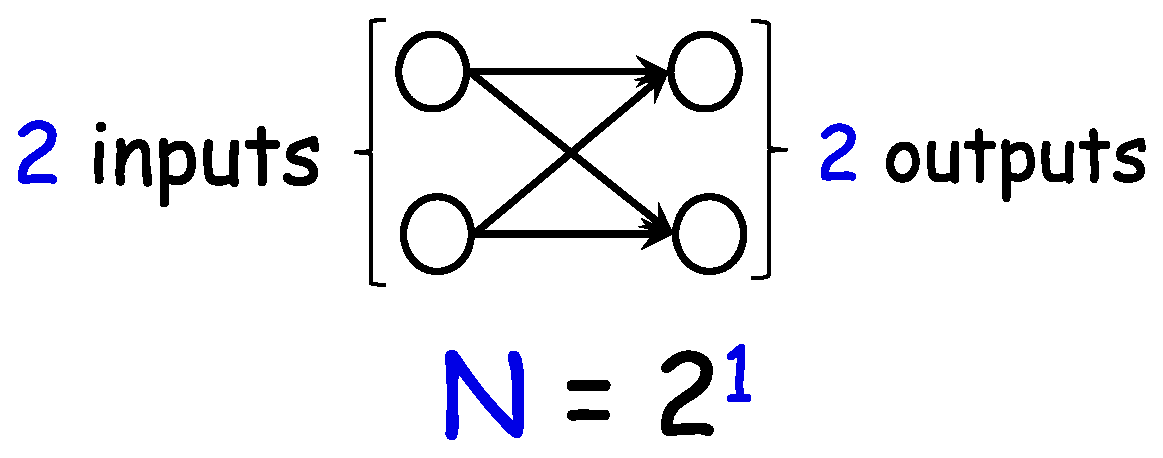
\includegraphics{figures/butterfly-base}
\end{center}
\caption{$F_1$, the Butterfly Net switches with $N=2^1$.}
\label{fig:butterfly-base}
\end{figure}

\begin{staffnotes}

The butterfly of size $2N$ consists of two butterflies of size $N$, which
are shown in dashed boxes below, and one additional level of switches.
Each switch in the new level has directed edges to a pair of
corresponding switches in the smaller butterflies; one example is
dashed in the figure.

\mfigure{!}{3in}{figures/butterfly3}

Despite the relatively complicated structure of the butterfly, there
is a simple way to route packets.  In particular, suppose that we want
to send a packet from input $x_1 x_2 \dots x_{\log N}$ to output $y_1
y_2 \dots y_{\log N}$.  (Here we are specifying the input and output
numbers in binary.)  Roughly, the plan is to ``correct'' the first bit
by level 1, correct the second bit by level 2, and so forth.  Thus,
the sequence of switches visited by the packet is:
%
\begin{align*}
(x_1, x_2, x_3, \dots, x_{\log N}, 0)
    & \to (y_1, x_2, x_3, \dots, x_{\log N}, 1) \\
    & \to (y_1, y_2, x_3, \dots, x_{\log N}, 2) \\
    & \to (y_1, y_2, y_3, \dots, x_{\log N}, 3) \\
    & \to \qquad \dots \\
    & \to (y_1, y_2, y_3, \dots, y_{\log N}, \log N) \\
\end{align*}
%
In fact, this is the \textit{only} path from the input to the output!

\end{staffnotes}

In the constructor step, we construct $F_{n+1}$ with $2^{n+1}$ inputs and
outputs out of two $F_n$ nets connected to a new set of $2^{n+1}$ input
switches, as shown in as in Figure~\ref{fig:butterfly-recursive}.  That
is, the $i$th and $2^n+i$th new input switches are each connected to the
same two switches, namely, to the $i$th input switches of each of two
$F_n$ components for $i=1,\dots,2^n$.  The output switches of $F_{n+1}$
are simply the output switches of each of the $F_n$ copies.

\begin{figure}[h]
\begin{center}
\mfigure{!}{3in}{figures/butterfly-recursive}
%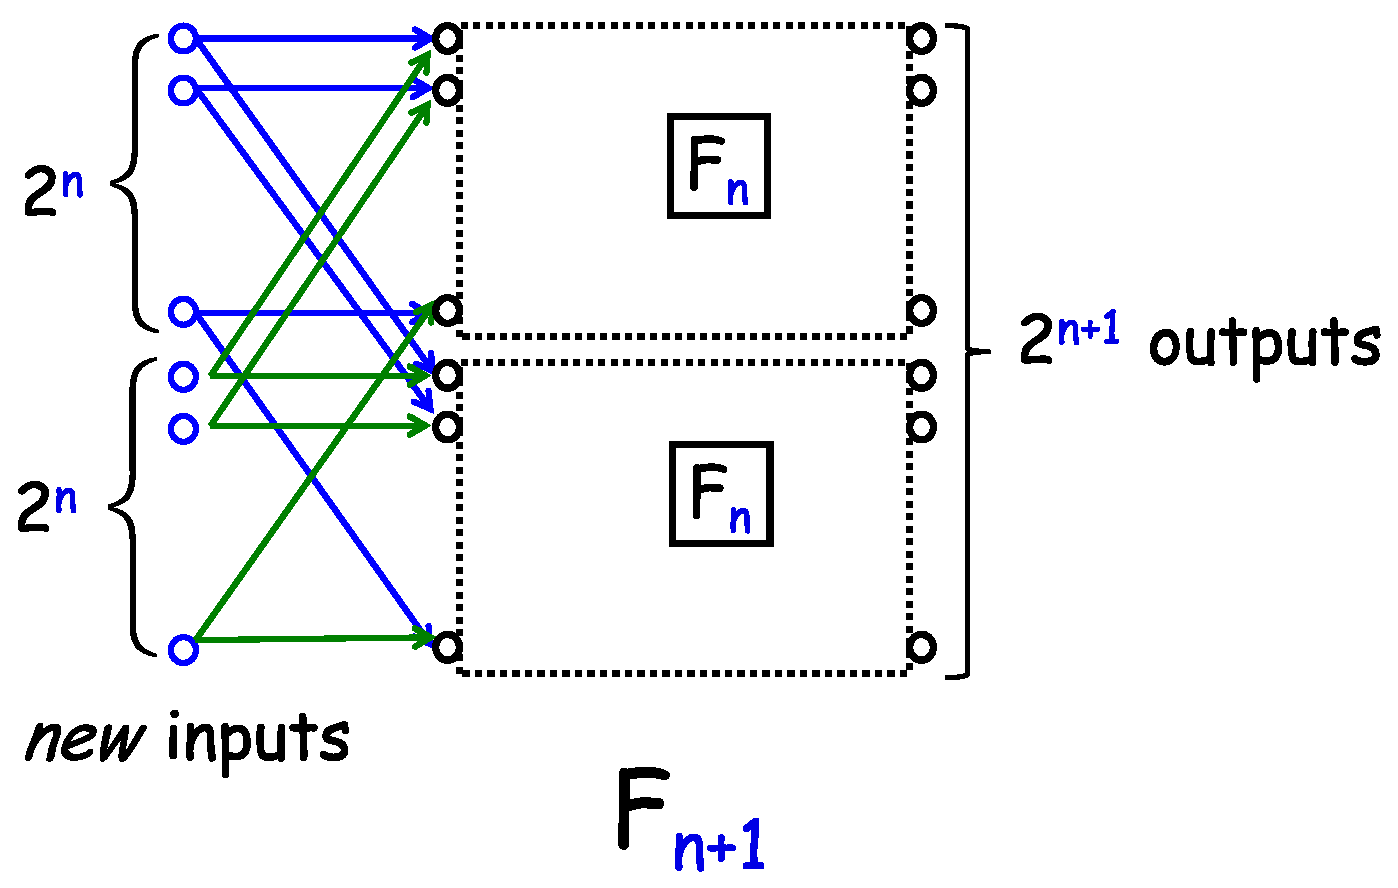
\includegraphics{figures/butterfly-recursive}
\end{center}
\caption{$F_{n+1}$, the Butterfly Net switches with $2^{n+1}$ inputs
and outputs.}
\label{fig:butterfly-recursive}
\end{figure}

So $F_{n+1}$ is laid out in columns of height $2^{n+1}$ by adding one more
column of switches to the columns in $F_n$.  Since the construction starts
with two columns when $n=1$, the $F_{n+1}$ switches are arrayed in $n+1$
columns.  The total number of switches is the height of the columns times
the number of columns, namely, $2^{n+1}(n+1)$.  Remembering that $n=\log
N$, we conclude that the Butterfly Net with $N$ inputs has $N(\log N +1)$
switches.

Since every path in $F_{n+1}$ from an input switch to an output is the
same length, namely, $n+1$, the diameter of the Butterfly net with
$2^{n+1}$ inputs is this length plus two because of the two edges
connecting to the terminals (square boxes) ---one edge from input
terminal to input switch (circle) and one from output switch to output
terminal.

There is an easy recursive procedure to route a packet through the
Butterfly Net.  In the base case, there is obviously only one way to route
a packet from one of the two inputs to one of the two outputs.  Now
suppose we want to route a packet from an input switch to an output switch
in $F_{n+1}$.  If the output switch is in the ``top'' copy of $F_n$, then
the first step in the route must be from the input switch to the unique
switch it is connected to in the top copy; the rest of the route is
determined by recursively routing the rest of the way in the top copy of
$F_n$.  Likewise, if the output switch is in the ``bottom'' copy of $F_n$,
then the first step in the route must be to the switch in the bottom copy,
and the rest of the route is determined by recursively routing in the
bottom copy of $F_n$.  In fact, this argument shows that the routing is
\emph{unique}: there is exactly one path in the Butterfly Net from each
input to each output, which implies that the network latency when
minimizing congestion is the same as the diameter.

The congestion of the butterfly network is about $\sqrt{N}$, more
precisely, the congestion is $\sqrt{N}$ if $N$ is an even power of 2 and
$\sqrt{N/2}$ if $N$ is an odd power of 2.  A simple proof of this appears
in Problem\ref{PS_butterfly_congestion}.

Let's add the butterfly data to our comparison table:
%
\[
\begin{array}{r|c|c|c|c}
\textbf{network} &
\textbf{diameter} &
\textbf{switch size} &
\textbf{\# switches} &
\textbf{congestion} \\ \hline
\text{complete binary tree} & 2 \log N + 2 & 3 \times 3 & 2N - 1 & N \\
\text{2-D array} & 2 N & 2 \times 2 & N^2 & 2 \\
\text{butterfly} & \log N + 2 & 2 \times 2 & N (\log(N) + 1) & \sqrt{N} \text{ or } \sqrt{N/2}
\end{array}
\]
%
The butterfly has lower congestion than the complete binary tree.  And
it uses fewer switches and has lower diameter than the array.
However, the butterfly does not capture the best qualities of each
network, but rather is a compromise somewhere between the two.  So our
quest for the Holy Grail of routing networks goes on.

\section{Bene\u{s} Network}

In the 1960's, a researcher at Bell Labs named Bene\u{s} had a
remarkable idea.  He obtained a marvelous communication network with
congestion 1 by placing \textit{two} butterflies back-to-back.  This
amounts to recursively growing \term{Bene\u{s} nets} by adding both inputs
and outputs at each stage.  Now we recursively define $B_n$ to be the
switches and connections (without the terminals) of the Bene\u{s} net
with $N \eqdef 2^n$ input and output switches.

The base case, $B_1$, with 2 input switches and 2 output switches is
exactly the same as $F_1$ in Figure~\ref{fig:butterfly-base}.

In the constructor step, we construct $B_{n+1}$ out of two $B_n$ nets
connected to a new set of $2^{n+1}$ input switches \emph{and also} a
new set of $2^{n+1}$ output switches.  This is illustrated in
Figure~\ref{fig:benes-recursive}.

Namely, the $i$th and $2^n+i$th new input switches are each connected to
the same two switches, namely, to the $i$th input switches of each of two
$B_n$ components for $i=1,\dots,2^n$, exactly as in the Butterfly net.  In
addition, the $i$th and $2^n+i$th new \emph{output} switches are connected
to the same two switches, namely, to the $i$th output switches of each of
two $B_n$ components.

\begin{figure}[h]
\begin{center}
\mfigure{!}{4in}{figures/benes-recursive}
%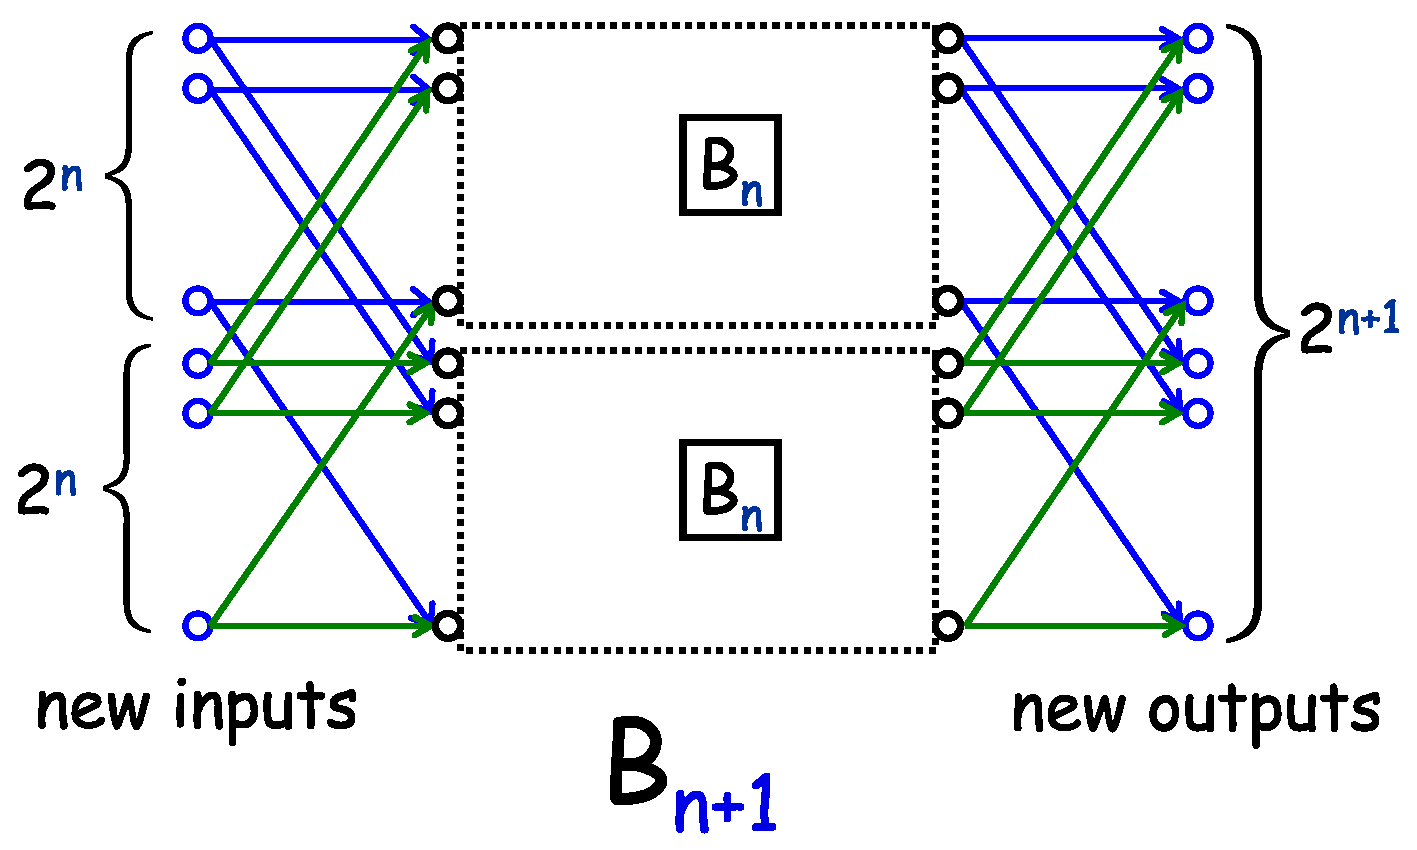
\includegraphics{figures/benes-recursive}
\end{center}
\caption{$B_{n+1}$, the Bene\u{s} Net switches with $2^{n+1}$ inputs
and outputs.}
\label{fig:benes-recursive}
\end{figure}

Now $B_{n+1}$ is laid out in columns of height $2^{n+1}$ by adding two
more columns of switches to the columns in $B_n$.  So the $B_{n+1}$
switches are arrayed in $2(n+1)$ columns.  The total number of
switches is the number of columns times the height of the columns,
namely, $2(n+1)2^{n+1}$.

All paths in $B_{n+1}$ from an input switch to an output are the same
length, namely, $2(n+1)-1$, and the diameter of the Bene\u{s} net with
$2^{n+1}$ inputs is this length plus two because of the two edges
connecting to the terminals.

\begin{staffnotes}

\mfigure{5in}{!}{figures/benes}

% This should make the construction of the 2-colorable graph in the
% congestion proof just a little more apparent.

This network now has levels labeled $0,\dots ,2 \log N + 1$. For $1 \leq k
\leq \log N$, the connections from level $k-1$ to level $k$ are just as in
the Butterfly network, the connections based on bit $k$. The conections
from level $2 \log N - k + 1$ to level $2 \log N - k + 2$ are also the
ones based on bit $k$.  (Informally, to make the connections from level
$0$ to level $2 \log N +1$ one level at a time, use the connections based
on bits $1,2,3,\dots, \log N - 1, \log N, \log N - 1, \log N - 2, \dots,
3,2,1$ in that order.)

\end{staffnotes}

So Bene\u{s} has doubled the number of switches and the diameter, of
course, but completely eliminates congestion problems!  The proof of
this fact relies on a clever induction argument that we'll come to in
a moment.  Let's first see how the Bene\u{s} network stacks up:
%
\[
\begin{array}{r|c|c|c|c}
\textbf{network} &
\textbf{diameter} &
\textbf{switch size} &
\textbf{\# switches} &
\textbf{congestion} \\ \hline
\text{complete binary tree} & 2 \log N + 2 & 3 \times 3 & 2N - 1 & N \\
\text{2-D array} & 2 N & 2 \times 2 & N^2 & 2 \\
\text{butterfly} & \log N + 2 & 2 \times 2 & N (\log(N) + 1) & \sqrt{N} \text{ or } \sqrt{N/2} \\
\text{Bene\u{s}} & 2 \log N + 1 & 2 \times 2 &  2 N \log N & 1
\end{array}
\]
%
The Bene\u{s} network has small size and diameter, and completely
eliminates congestion.  The Holy Grail of routing networks is in hand!

\begin{theorem}
The congestion of the $N$-input Bene\u{s} network is 1.

\iffalse , where $N = 2^a$ for some $a \geq 1$\fi

\end{theorem}

\begin{proof}
By induction on $n$ where $N=2^n$.  So the induction hypothesis is

\[
P(n) \eqdef  \text{the congestion of $B_n$ is 1}.
\]

\textbf{Base case} ($n=1$): $B_1 =F_1$ and the unique routings in $F_1$
have congestion 1.

\textbf{Inductive step}: We assume that the congestion of an $N=2^n$-input
Bene\u{s} network is 1 and prove that the congestion of a $2N$-input
Bene\u{s} network is also 1.

\textbf{Digression. }  Time out!  Let's work through an example,
develop some intuition, and then complete the proof.  In the Bene\u{s}
network shown below with $N=8$ inputs and outputs, the two
4-input/output subnetworks are in dashed boxes.

\mfigure{!}{3in}{figures/benes-decomp}

By the inductive assumption, the subnetworks can each route an
arbitrary permutation with congestion 1.  So if we can guide packets
safely through just the first and last levels, then we can rely on
induction for the rest!  Let's see how this works in an example.
Consider the following permutation routing problem:
%
\begin{align*}
\pi(0) & = 1 & \pi(4) & = 3 \\
\pi(1) & = 5 & \pi(5) & = 6 \\
\pi(2) & = 4 & \pi(6) & = 0 \\
\pi(3) & = 7 & \pi(7) & = 2
\end{align*}

We can route each packet to its destination through either the upper
subnetwork or the lower subnetwork.  However, the choice for one
packet may constrain the choice for another.  For example, we can not
route both packet 0 \textit{and} packet 4 through the same network
since that would cause two packets to collide at a single switch,
resulting in congestion.  So one packet must go through the upper
network and the other through the lower network.  Similarly, packets 1
and 5, 2 and 6, and 3 and 7 must be routed through different networks.
Let's record these constraints in a graph.  The vertices are the 8
packets.  If two packets must pass through different networks, then
there is an edge between them.  Thus, our constraint graph looks like
this:

\mfigure{!}{1.5in}{figures/benes-const1}

Notice that at most one edge is incident to each vertex.

The output side of the network imposes some further constraints.  For
example, the packet destined for output 0 (which is packet 6) and the
packet destined for output 4 (which is packet 2) can not both pass
through the same network; that would require both packets to arrive
from the same switch.  Similarly, the packets destined for outputs 1
and 5, 2 and 6, and 3 and 7 must also pass through different switches.
We can record these additional constraints in our graph with gray
edges:

\mfigure{!}{1.5in}{figures/benes-const2}

Notice that at most one new edge is incident to each vertex.
The two lines drawn between vertices 2 and 6 reflect the two different
reasons why these packets must be routed through different networks.
However, we intend this to be a simple graph; the two lines still
signify a single edge.

Now here's the key insight: \textit{a 2-coloring of the graph
corresponds to a solution to the routing problem}.  In particular,
suppose that we could color each vertex either red or blue so that
adjacent vertices are colored differently.  Then all constraints are
satisfied if we send the red packets through the upper network and the
blue packets through the lower network.

The only remaining question is whether the constraint graph is
2-colorable, which is easy to verify:

\begin{lemma}\label{deg1-union}
  Prove that if the edges of a graph can be grouped into two sets such
  that every vertex has at most 1 edge from each set incident to it, then
  the graph is 2-colorable.
\end{lemma}

\begin{proof}
  Since the two sets of edges may overlap, let's call an edge that is in
  both sets a \emph{doubled edge}.

  We know from Theorem~\ref{odd-cycle} that all we have to do is show that
  every cycle has even length.  There are two cases:

  \textbf{Case 1}: [The cycle contains a doubled edge.]  No other edge can
  be incident to either of the endpoints of a doubled edge, since that
  endpoint would then be incident to two edges from the same set.  So a
  cycle traversing a doubled edge has nowhere to go but back and forth
  along the edge an even number of times.

  \textbf{Case 2}: [No edge on the cycle is doubled.]  Since each vertex
  is incident to at most one edge from each set, any path with no doubled
  edges must traverse successive edges that alternate from one set to the
  other.  In particular, a cycle must traverse a path of alternating edges
  that begins and ends with edges from different sets.  This means the
  cycle has to be of even length.
\end{proof}

For example, here is a 2-coloring of the constraint graph:

\mfigure{!}{1.75in}{figures/benes-const3}

The solution to this graph-coloring problem provides a start
on the packet routing problem:

We can complete the routing in the two smaller Bene\u{s} networks by
induction!  Back to the proof.  \textbf{End of Digression.}

Let $\pi$ be an arbitrary permutation of $\set{0, 1, \dots, N-1}$.  Let $G$
be the graph whose vertices are packet numbers $0, 1, \dots, N-1$ and whose edges
come from the union of these two sets:
\begin{align*}
E_1 \eqdef &  \set{\edge{u}{v} \suchthat \abs{u - v} = N/2},\ \text{and} \\
E_2 \eqdef &  \set{\edge{u}{w} \suchthat \abs{\pi(u) - \pi(w)} = N/2}.
\end{align*}
Now any vertex, $u$, is incident to at most two edges: a unique edge
$\edge{u}{v} \in E_1$ and a unique edge $\edge{u}{w} \in E_2$.  So
according to Lemma~\ref{deg1-union}, there is a 2-coloring for the
vertices of $G$.  Now route packets of one color through the upper
subnetwork and packets of the other color through the lower subnetwork.
Since for each edge in $E_1$, one vertex goes to the upper subnetwork and
the other to the lower subnetwork, there will not be any conflicts in the
first level.  Since for each edge in $E_2$, one vertex comes from the
upper subnetwork and the other from the lower subnetwork, there will not
be any conflicts in the last level.  We can complete the routing within
each subnetwork by the induction hypothesis $P(n)$.
\end{proof}

\begin{problems}
\examproblems
\pinput{MQ_basic_network_problem}

\classproblems
\pinput{CP_Benes_network}
\pinput{CP_binary-tree_network}
\pinput{CP_2_layer_array_network}
\pinput{CP_n-path_network}
\pinput{CP_Megumi_net}

\homeworkproblems
\pinput{PS_Reasoner_net}
\pinput{PS_butterfly_congestion}
\end{problems}

\iffalse
In class, you will work through an example in which you route packets
using this recursive idea!
\fi

\endinput

